\documentclass[tikz,border=2pt]{standalone}
% Preámbulo común de los diagramas TikZ (misma paleta y letra que las notas)
\usepackage[T1]{fontenc}\usepackage[utf8]{inputenc}
\usepackage{libertinus}\usepackage{libertinust1math}
\usepackage[defaultsans,scale=0.92]{lato}
\usepackage{amsmath,amssymb,bm}
\usepackage{tikz}\usetikzlibrary{calc,positioning,arrows.meta,shapes.geometric,decorations.pathreplacing,decorations.pathmorphing,fit,backgrounds}
\definecolor{snlazul}{HTML}{1E5AA8}\definecolor{snlnoche}{HTML}{14213D}\definecolor{snlvioleta}{HTML}{6C4AB6}
\definecolor{snlcoral}{HTML}{D1495B}\definecolor{snlambar}{HTML}{E09F3E}\definecolor{snlverde}{HTML}{2A9D8F}
\definecolor{snlteal}{HTML}{0F7173}\definecolor{snlgris}{HTML}{5C677D}\definecolor{snlfondo}{HTML}{F4F6FA}
\tikzset{>={Stealth[length=2.2mm]},
  bloque/.style={draw=#1,fill=#1!8,thick,rounded corners=2pt,minimum height=11mm,minimum width=20mm,align=center,font=\small},
  bloque/.default=snlazul,
  suma/.style={draw=snlnoche,thick,circle,inner sep=0pt,minimum size=5mm},
  flecha/.style={->,thick,draw=snlnoche},
  etq/.style={font=\small,text=snlnoche},
  nota/.style={font=\footnotesize\sffamily,text=snlgris,align=center}}

\begin{document}
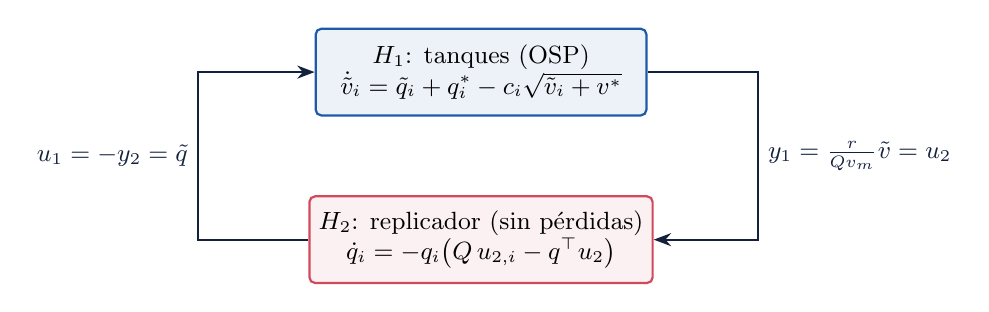
\begin{tikzpicture}
 \node[bloque=snlazul,minimum width=42mm] (H1) {$H_1$: tanques (OSP)\\$\dot{\tilde v}_i=\tilde q_i+q_i^*-c_i\sqrt{\tilde v_i+v^*}$};
 \node[bloque=snlcoral,below=10mm of H1,minimum width=42mm] (H2) {$H_2$: replicador (sin pérdidas)\\$\dot q_i=-q_i\bigl(Q\,u_{2,i}-q^\top u_2\bigr)$};
 \draw[flecha] (H1.east) -- ++(14mm,0) |- node[pos=0.25,right,etq]{$y_1=\tfrac{r}{Qv_m}\tilde v=u_2$} (H2.east);
 \draw[flecha] (H2.west) -- ++(-14mm,0) |- node[pos=0.25,left,etq]{$u_1=-y_2=\tilde q$} (H1.west);
\end{tikzpicture}
\end{document}
